\section{Metodi non lineari}\label{sec:non-linear}

Nella sezione \ref{sec:linear-model} sono stati introdotti ed adottati dei
metodi di regressione lineare che fornivano dei risultati discreti in prima
analisi, ma che possono essere sostituiti con modelli non lineari che spiegano
ancora meglio i dati.

A tal fine, sono stati provati vari modelli, descritti nelle sottosezioni
seguenti.

%%%%%%%%%%%%%%%%%%%%%%%%%%%%%%%%%%%%%%%%%%%%%%%%%%%%%%%%%%%%%%%%%%%%%%%%%%%%%%%

\subsection{Regressione locale}\label{sec:local-regression}
Come primo modello non lineare si sceglie di utilizzare la regressione locale,
servendosi del package \texttt{sm} presente in R.

In questo caso ci si limita a eseguire la regressione locale solamente per le
due variabili \texttt{datetime} e \texttt{temp}, le quali ci si aspettava che
fossero più importanti per la richiesta del servizio di \emph{Bike sharing};
tale ipotesi è stata verificata grazie al modello lineare, in cui queste
variabili erano risultate più significative sia nella scala logaritmica che in
quella originale.

Oltre a questo, la regressione locale viene svolta solamente per la scala
logaritmica, poichè si ritiene che riesca a modellare meglio il sistema in
esame.

\paragraph{Scelta di \emph{h}} \mbox{}\\
Per questo modello era importante scegliere il parametro \emph{h}, che regola
l'ampiezza della finestra di lisciamento.

Per la scelta del parametro, gli script \texttt{mySM\_temp.R} (sez.
\ref{sec:mySM-temp}) e lo script \texttt{mySM\_datetime.R} (non riportato
perchè pressochè uguale a quello per la variabile \texttt{temp}) sono stati
fatti girare più volte, ottenendo ogni volta una misura ottimale di h e
restringendo l'intervallo attorno al valore salvato in \texttt{optimal\_h}.

Di seguito viene riportato l'andamento dell'errore in funzione di h:

\begin{figure}[H]
  \centering
  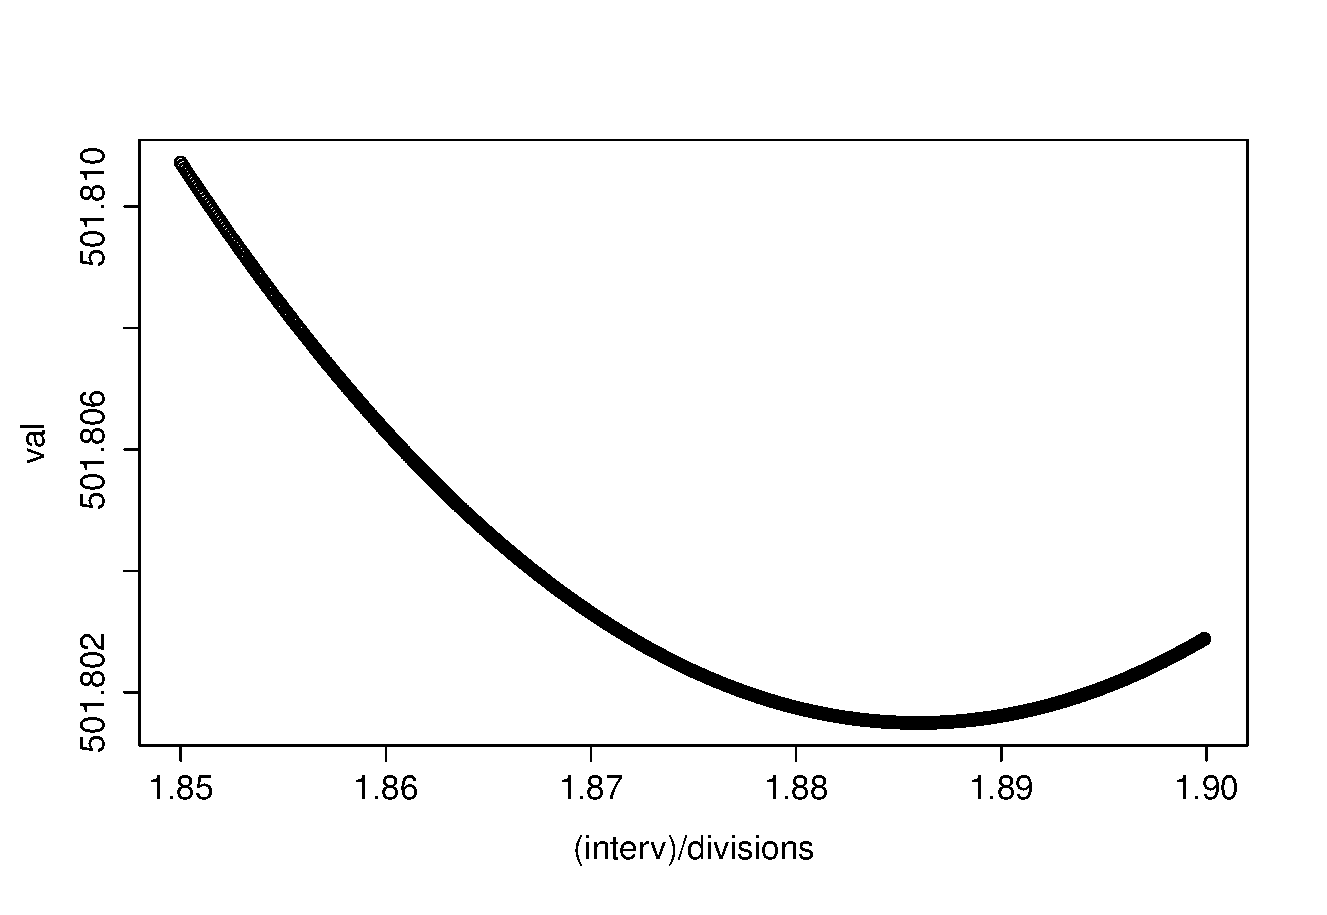
\includegraphics[width=.7\columnwidth]{images/non-linear/sm-optimal-h.eps}
  \caption{Curva dell'errore in funzione del parametro h}
  \label{fig:sm-optimal-h}
\end{figure}

Una volta iterato il procedimento fino ad avere una precisione per l'h
``ottimo'' migliore di $ \frac{1}{1000} $, si procede a disegnare la curva
grazie allo script \texttt{drawOptimalSM\_temp.R} (sez. \ref{sec:drawSM-temp}):

\begin{figure}[H]
  \centering
  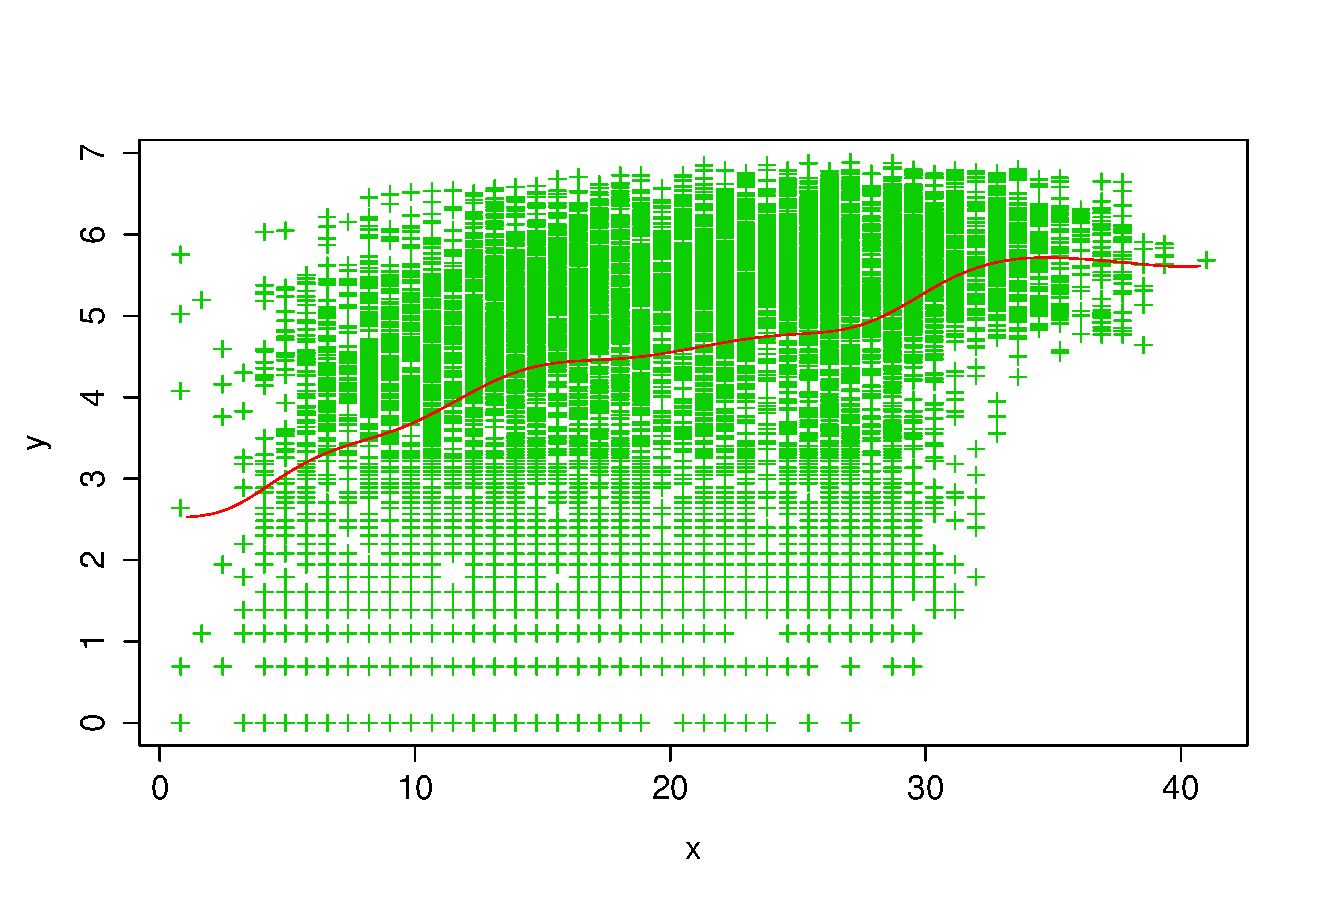
\includegraphics[width=.7\columnwidth]{images/non-linear/sm-draw.eps}
  \caption{Curva di regressione locale disegnata con il miglior h}
  \label{fig:sm-draw}
\end{figure}

%%%%%%%%%%%%%%%%%%%%%%%%%%%%%%%%%%%%%%%%%%%%%%%%%%%%%%%%%%%%%%%%%%%%%%%%%%%%%%%

\subsection{Loess}\label{sec:loess}
Un metodo molto simile al precedente, sempre di regressione locale, è il
\emph{loess}.

Questa tecnica permette di attenuare gli effetti degli \emph{outliers}, poichè
considera un intorno di k \emph{punti} e non un intorno di \emph{ampiezza} h.
Grazie a questa sua particolarità, il \emph{loess} è ritenuto un estimatore
\textbf{robusto}.

Tuttavia, anche questa tecnica viene eseguita con poche variabili alla volta;
sebbene il numero massimo di \emph{covariates} che il comando \texttt{loess}
di R accetta sia 4, si ritiene che eseguire la regressione locale con una
sola variabile esplicativa ne favorisca interpretazione.

Gli script utilizzati sono \texttt{loess\_temp.R} (sez. \ref{sec:loess-temp})
ed altri script non riportati perchè sostanzialmente identici a questo. In
tali procedure viene generato un insieme di addestramento e uno di verifica,
per poi cercare l'\texttt{optimal\_span} (la percentuale per la quale la somma
dei quadrati dei residui è minima).

\begin{figure}[H]
  \centering
  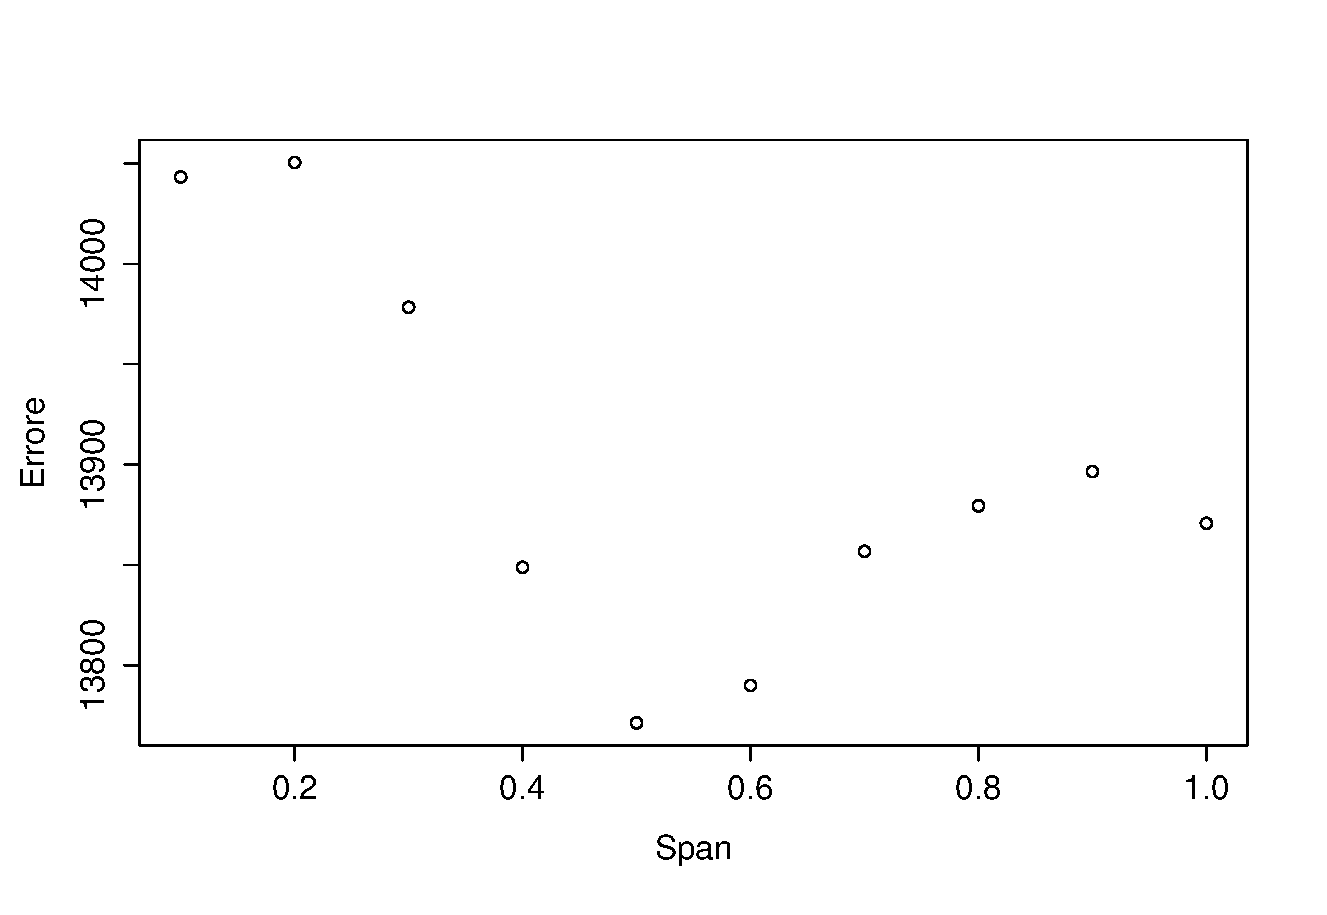
\includegraphics[width=.7\columnwidth]{images/non-linear/loess-error-span.eps}
  \caption{Curva dell'errore in funzione del parametro span}
  \label{fig:loess-optimal-span}
\end{figure}

\begin{figure}[H]
  \centering
  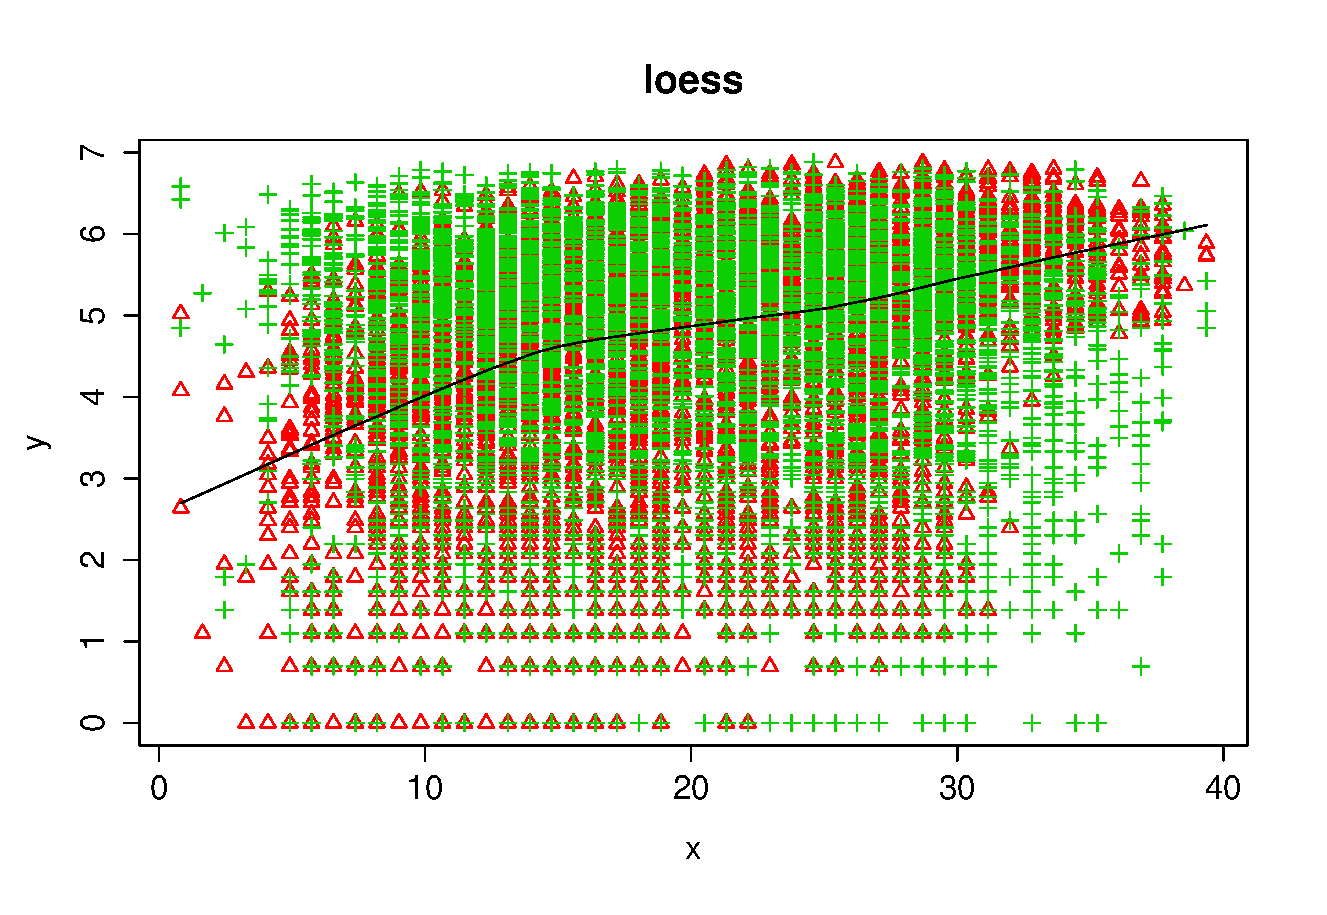
\includegraphics[width=.7\columnwidth]{images/non-linear/loess-draw.eps}
  \caption{Curva loess disegnata con il miglior span}
  \label{fig:loess-draw}
\end{figure}

%%%%%%%%%%%%%%%%%%%%%%%%%%%%%%%%%%%%%%%%%%%%%%%%%%%%%%%%%%%%%%%%%%%%%%%%%%%%%%%

\subsection{Spline di regressione}\label{sec:regression-splines}
Finora sono stati usati solamente modelli che, lineari o meno, erano costituiti
da una o più rette di regressione.

Con le spline si passa a curve che hanno tratti definiti da polinomi di grado
maggiore al primo: più precisamente, nel nostro caso verranno utilizzate
spline cubiche (con tratti definiti da polinomi di terzo grado).

Gli script che realizzano queste curve sono \texttt{regression-splines-temp.R}
(sez. \ref{sec:regression-splines-temp}) ed altri script non riportati perchè
sostanzialmente identici a questo.

Tali procedure utilizzano il comando \texttt{bs} di R, che genera spline con la
possibilità di impostare grado e numero di nodi.

\begin{figure}[H]
  \centering
  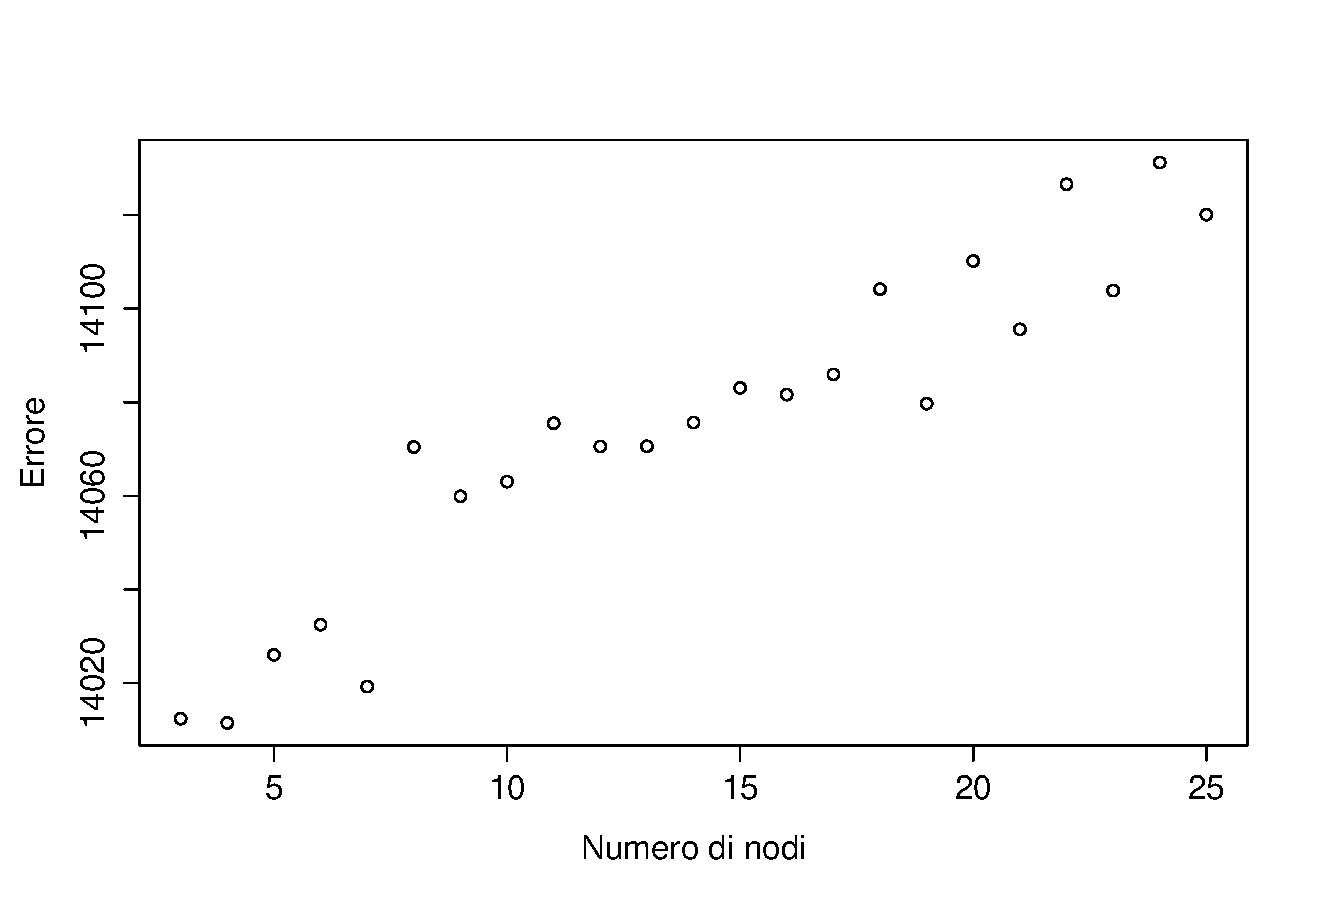
\includegraphics[width=.7\columnwidth]{images/non-linear/regression-splines-error-knots.eps}
  \caption{Curva dell'errore in funzione del numero di nodi}
  \label{fig:regression-optimal-knots}
\end{figure}

\begin{figure}[H]
  \centering
  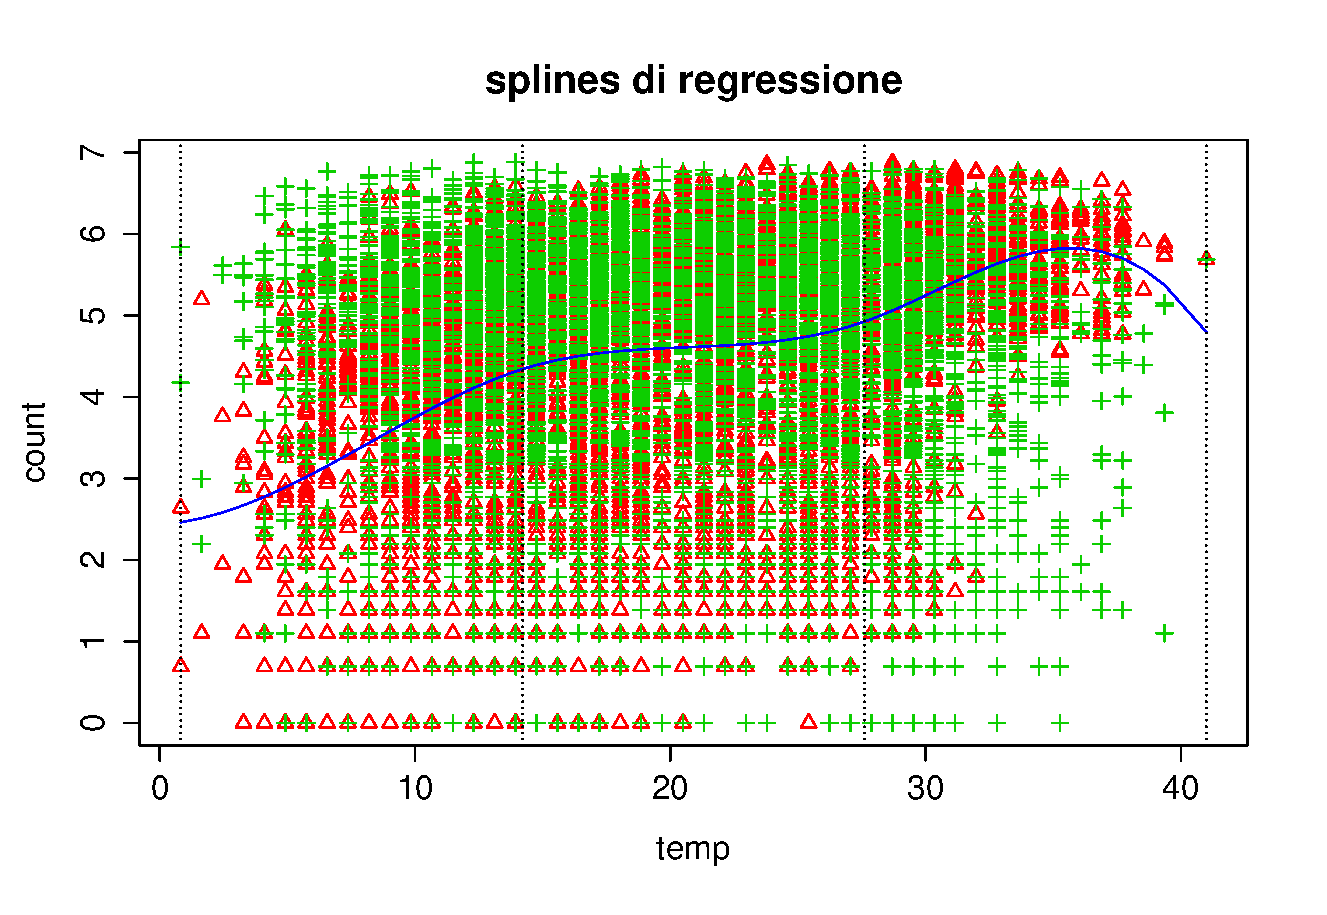
\includegraphics[width=.7\columnwidth]{images/non-linear/regression-draw.eps}
  \caption{Spline di regressione disegnata con il miglior numero di nodi}
  \label{fig:regression-draw}
\end{figure}

%%%%%%%%%%%%%%%%%%%%%%%%%%%%%%%%%%%%%%%%%%%%%%%%%%%%%%%%%%%%%%%%%%%%%%%%%%%%%%%

\subsection{Spline di lisciamento}\label{sec:smoothing-splines}
A differenza delle spline di regressione, che agivano sull'intera funzione,
possiamo anche introdurre un modello di regressione locale non lineare, ovvero
le \emph{spline di lisciamento}.

In un modo simile a quello visto per le spline di regressione, vengono
ottenute tante spline, una per ognuno degli intervalli scelti.

In questo caso, gli script utilizzati per ottenere il relativo modello sono
\texttt{smoothing-splines-temp.R} (sez. \ref{sec:smoothing-splines-temp}) ed
altri script non riportati perchè sostanzialmente identici a questo.

Tali procedure iterano affinchè non viene trovato il miglior valore di
$ \lambda $, ovvero il parametro di lisciamento utilizzato per tale modello (
$ \lambda = 0 \rightarrow $ funzione frastagliata,
$ \lambda = \infty \rightarrow $ regressione lineare semplice).

\begin{figure}[H]
  \centering
  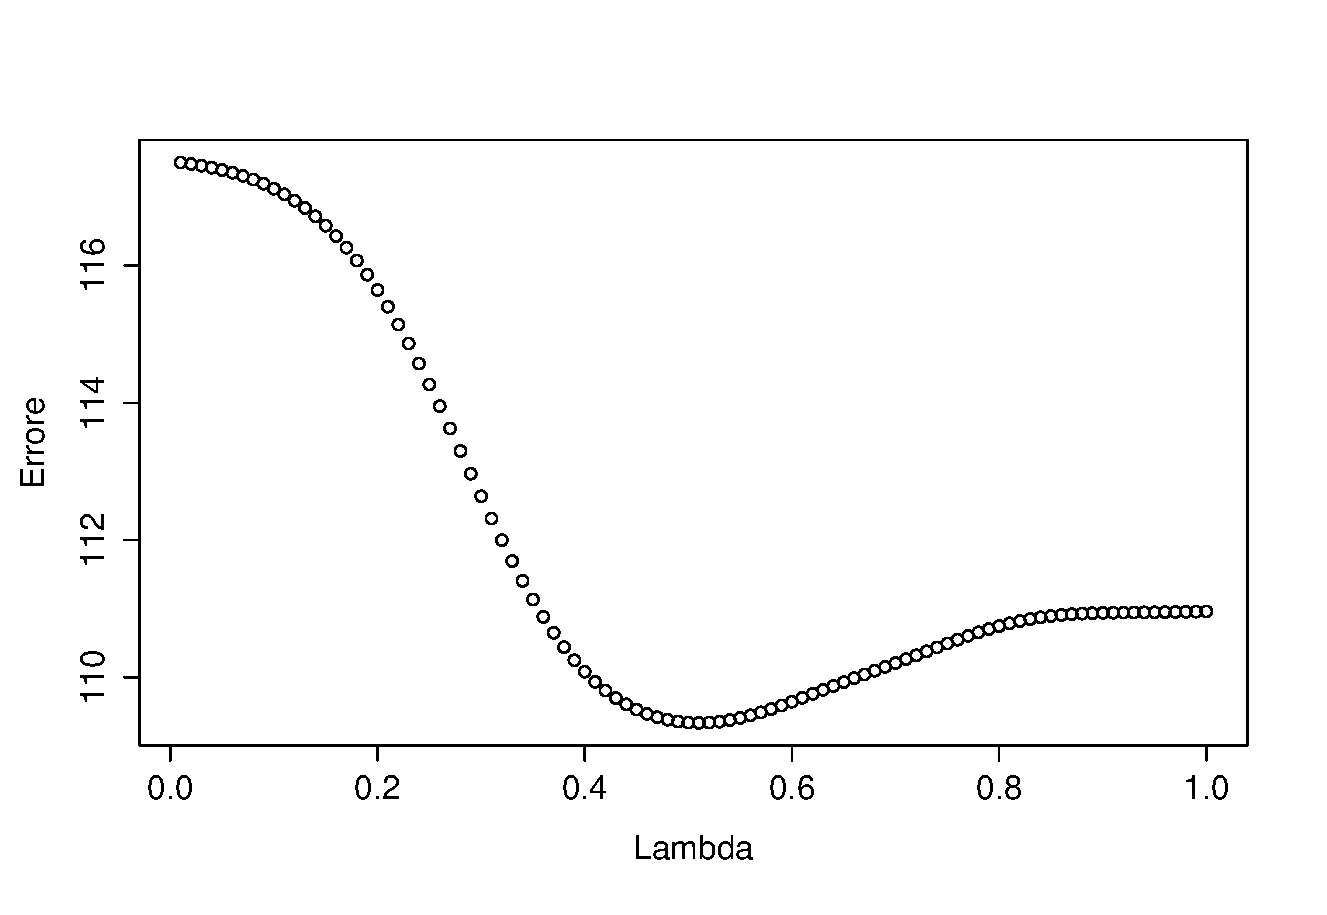
\includegraphics[width=.7\columnwidth]{images/non-linear/smoothing-splines-error-lambda.eps}
  \caption{Curva dell'errore in funzione di $ \lambda $}
  \label{fig:smoothing-optimal-lambda}
\end{figure}

\begin{figure}[H]
  \centering
  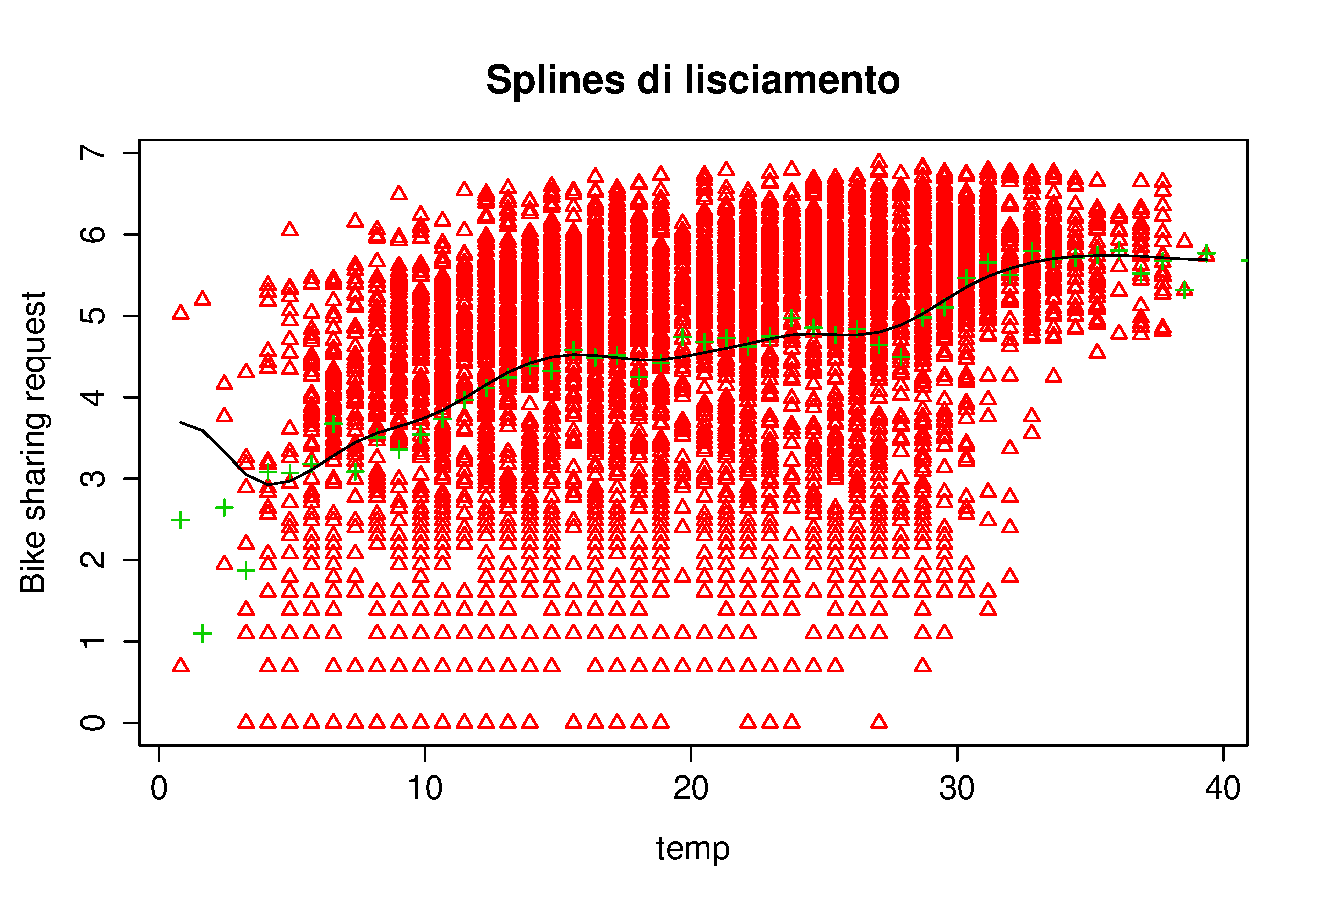
\includegraphics[width=.7\columnwidth]{images/non-linear/smoothing-spl-draw.eps}
  \caption{Spline di lisciamento disegnata con il miglior $ \lambda $}
  \label{fig:smoothing-spline-draw}
\end{figure}

%%%%%%%%%%%%%%%%%%%%%%%%%%%%%%%%%%%%%%%%%%%%%%%%%%%%%%%%%%%%%%%%%%%%%%%%%%%%%%%

\subsection{MARS}\label{sec:mars}
Oltre alle tecniche viste nelle sezioni \ref{sec:regression-splines} e
\ref{sec:smoothing-splines} vi è un ulteriore tecnica che utilizza le spline,
ovvero MARS (\emph{Multivariate Adaptive Regression Splines}).

Come dice il nome (esteso), grazie a questa tecnica è possibile utilizzare le
splines di regressione non solo più con un'unica variabile, ma con tutte le
variabili esplicative del dataset.

Lo script utilizzato per MARS è \texttt{mars.R}, presente in sezione
\ref{sec:mars-script}.

%%%%%%%%%%%%%%%%%%%%%%%%%%%%%%%%%%%%%%%%%%%%%%%%%%%%%%%%%%%%%%%%%%%%%%%%%%%%%%%

\subsection{GAM}\label{sec:gam}
Tutti i modelli visti finora soffrivano fortemente della ``maledizione della
dimensionalità'': al crescere di p (numero di variabili coinvolte e/o grado del
polinomio) l'errore cresce rapidamente a causa dell'\emph{overfitting}.

Con i GAM (\emph{Generalized Additive Model}) questo problema viene risolto
grazie a una struttura più flessibile del modello.

Lo script utilizzato è \texttt{gam.R}, presente nella sezione
\ref{sec:gam-script}. Di seguito vengono riportate le stime per le varie
variabili esplicative utilizzate nel modello.

\begin{figure}[H]
        \begin{subfigure}{0.4\textwidth}
          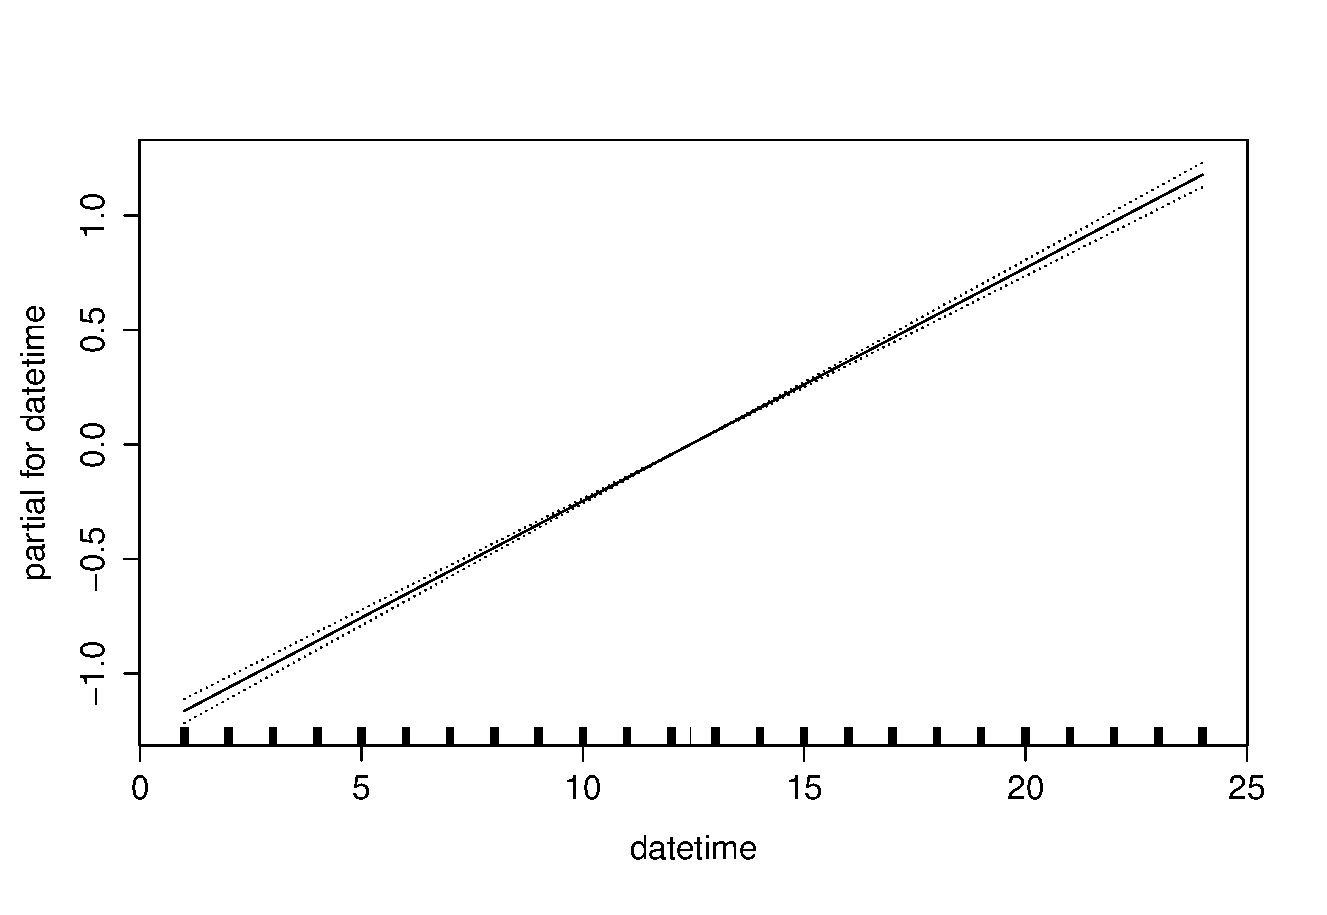
\includegraphics[width=\columnwidth]{images/non-linear/gam/gam-datetime.eps}
        \end{subfigure}
        \hspace*{\fill}
        \begin{subfigure}{0.4\textwidth}
          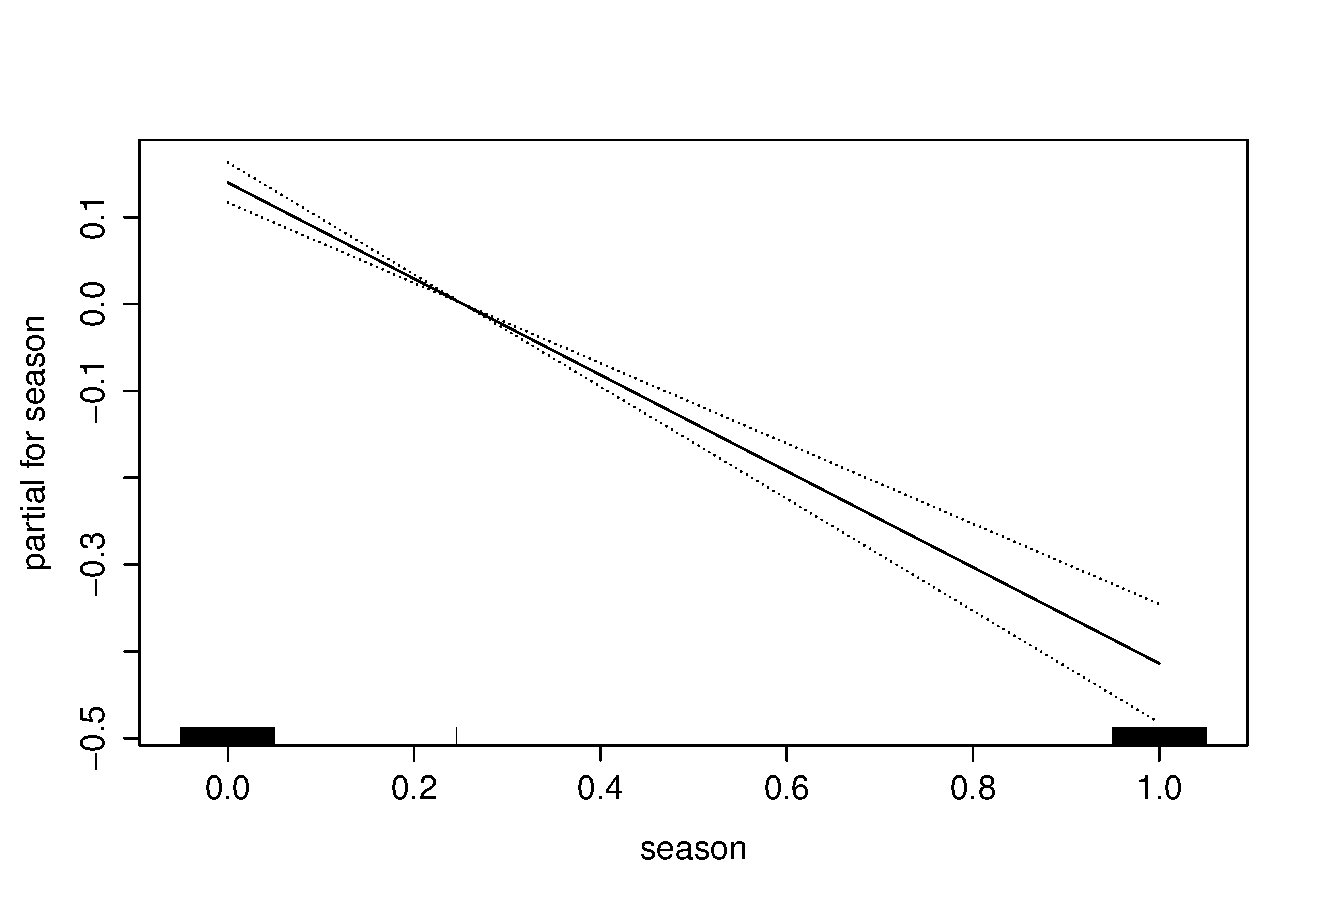
\includegraphics[width=\columnwidth]{images/non-linear/gam/gam-season.eps}
        \end{subfigure}

        \medskip
        \begin{subfigure}{0.4\textwidth}
          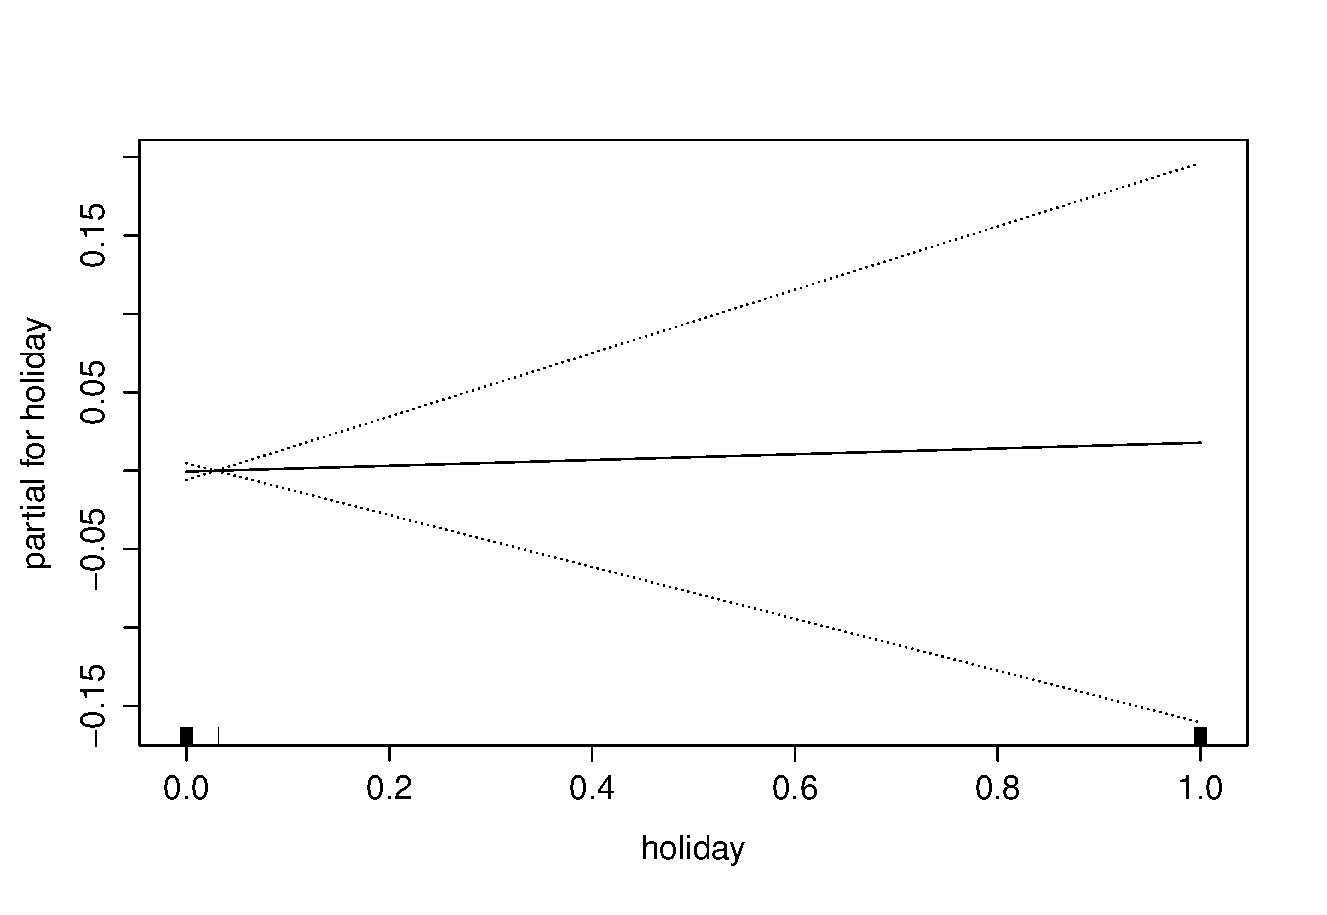
\includegraphics[width=\columnwidth]{images/non-linear/gam/gam-holiday.eps}
        \end{subfigure}
        \hspace*{\fill}
        \begin{subfigure}{.4\textwidth}
          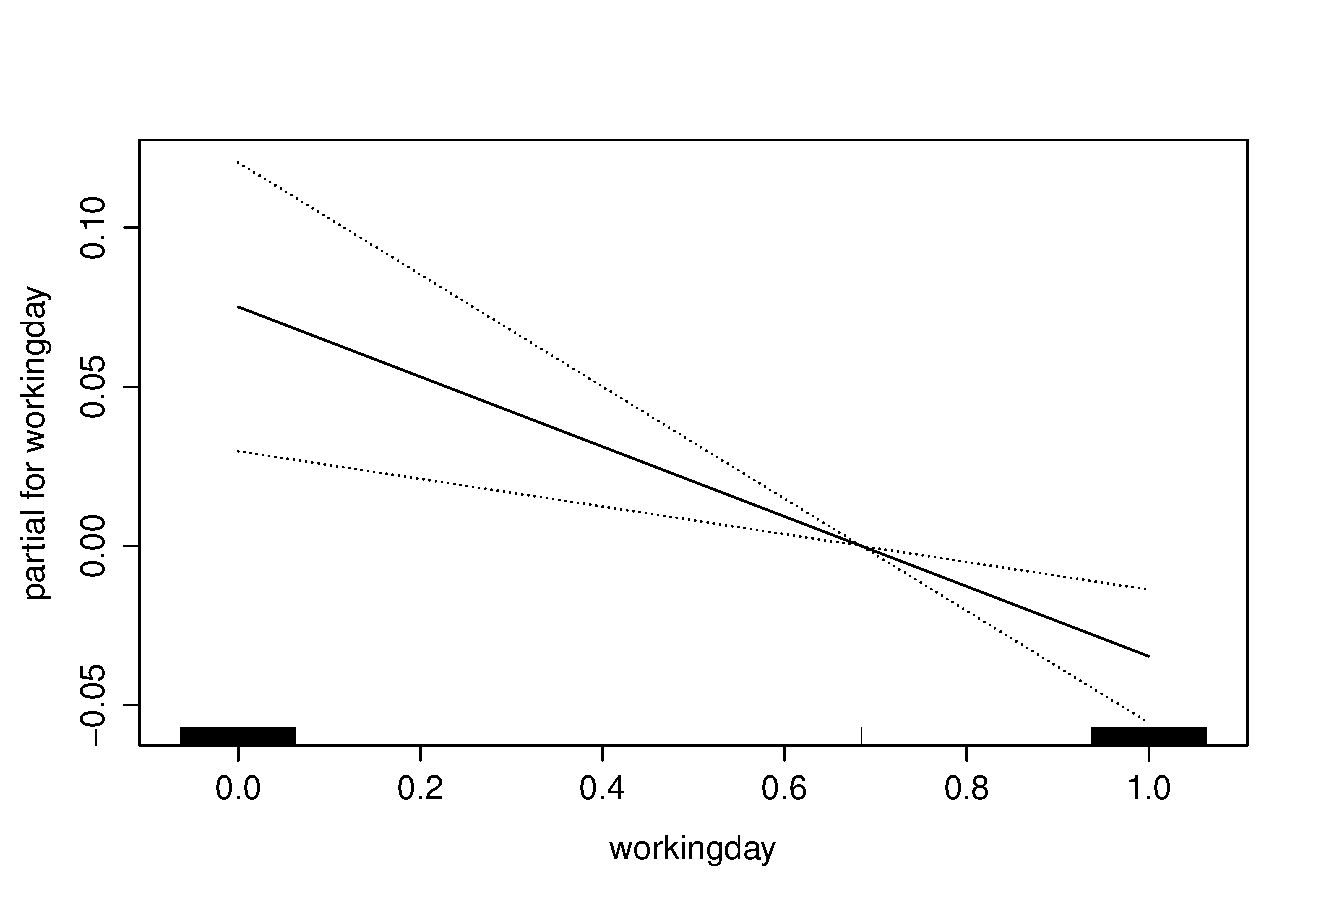
\includegraphics[width=\columnwidth]{images/non-linear/gam/gam-working-day.eps}
        \end{subfigure}

        \medskip
        \begin{subfigure}{0.4\textwidth}
          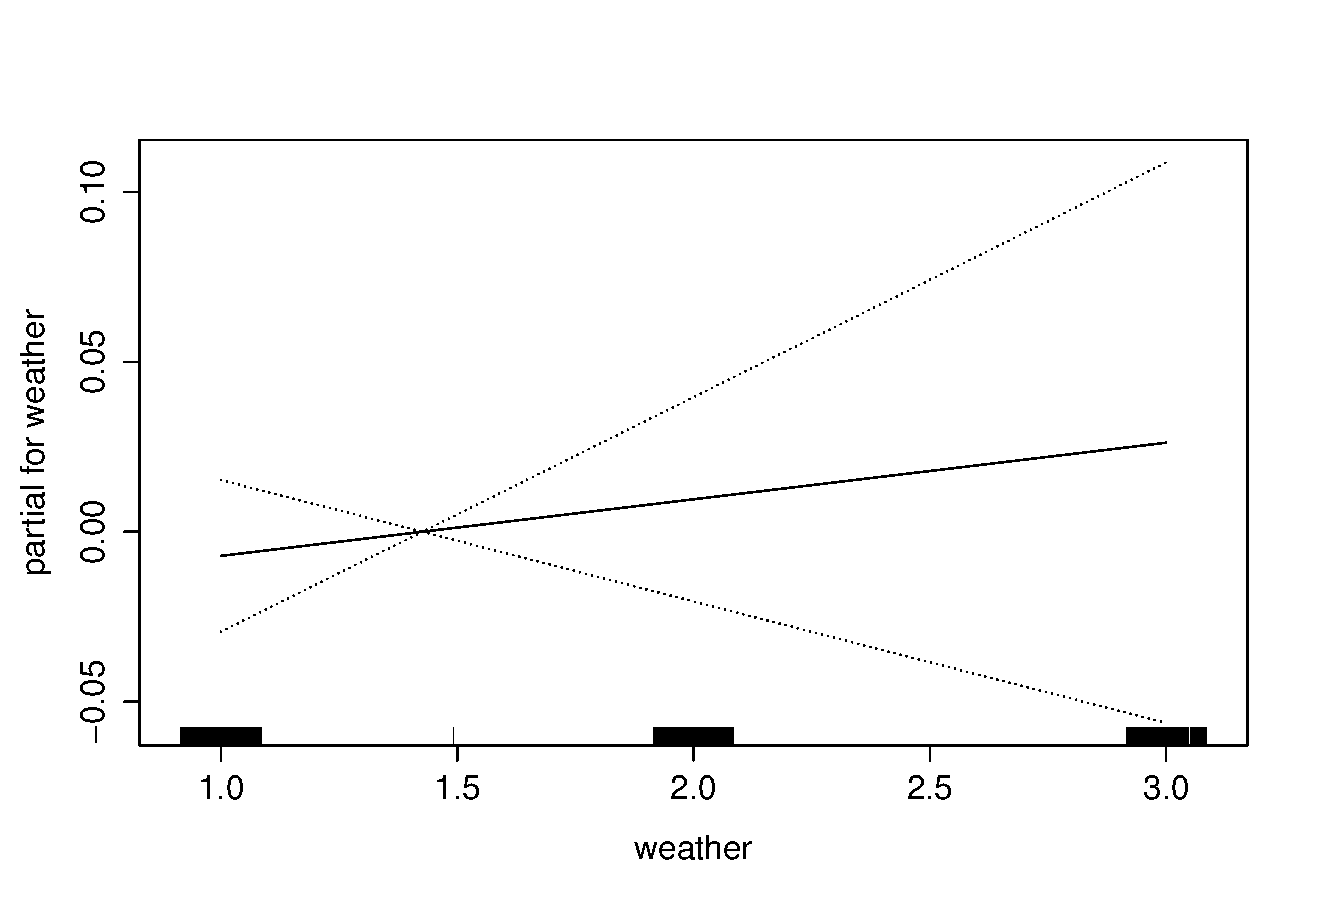
\includegraphics[width=\columnwidth]{images/non-linear/gam/gam-weather.eps}
        \end{subfigure}
        \hspace*{\fill}
        \begin{subfigure}{0.4\textwidth}
          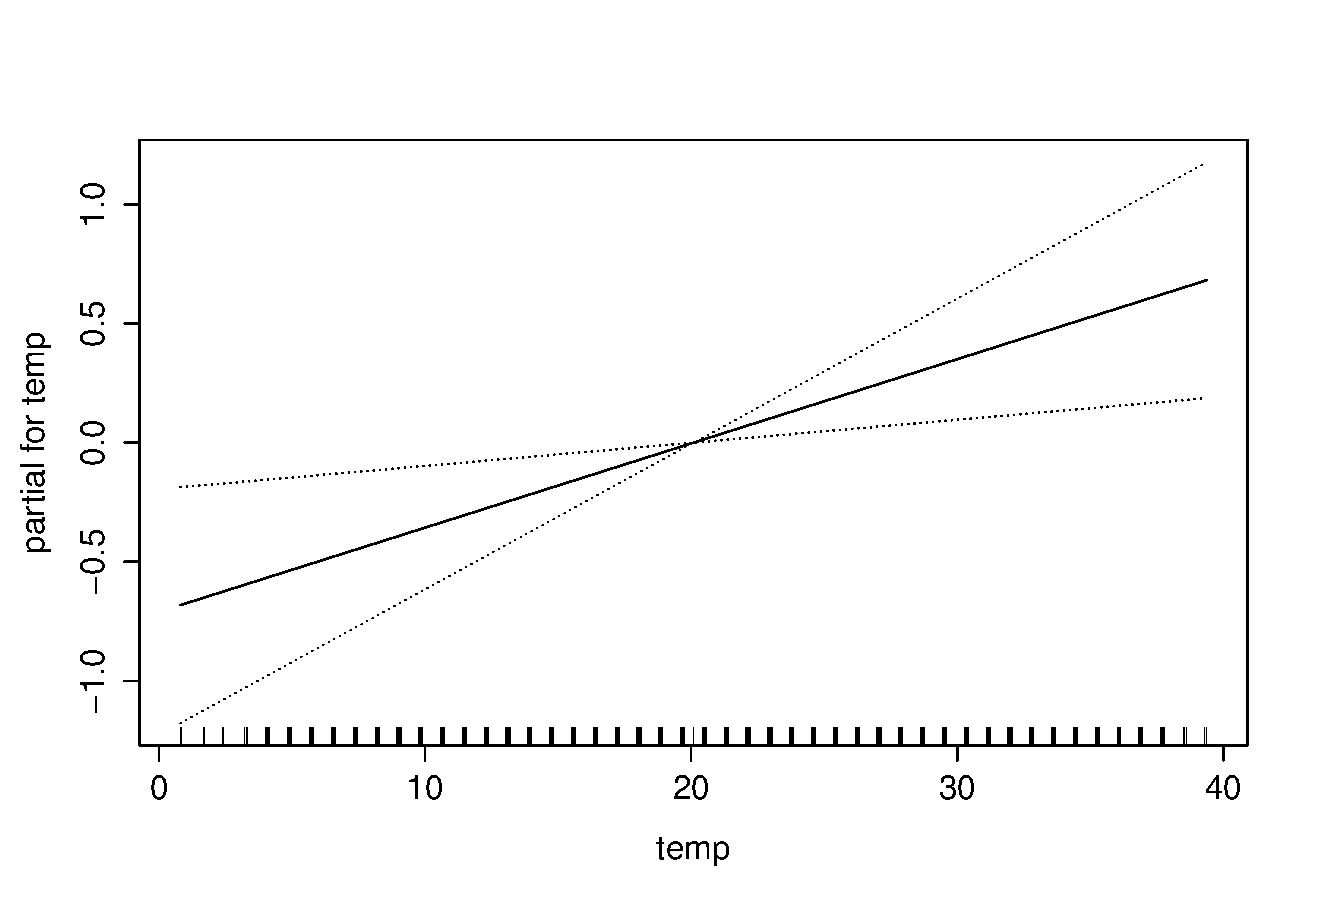
\includegraphics[width=\columnwidth]{images/non-linear/gam/gam-temp.eps}
        \end{subfigure}

        \caption{Grafici GAM - 1}\label{fig:gam-1}
\end{figure}

\begin{figure}[H]
        \begin{subfigure}{0.4\textwidth}
          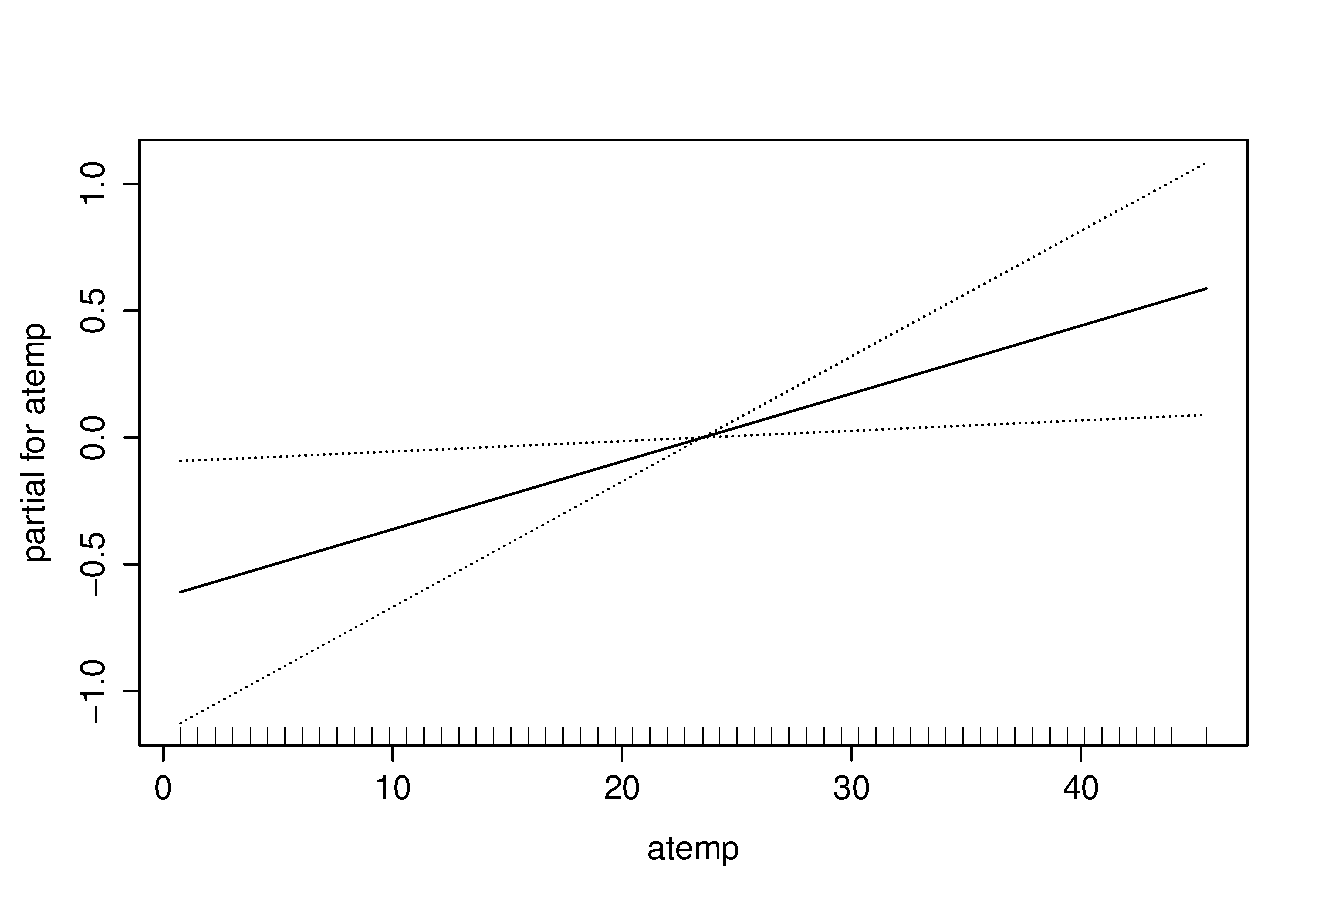
\includegraphics[width=\columnwidth]{images/non-linear/gam/gam-atemp.eps}
        \end{subfigure}
        \hspace*{\fill}
        \begin{subfigure}{0.4\textwidth}
          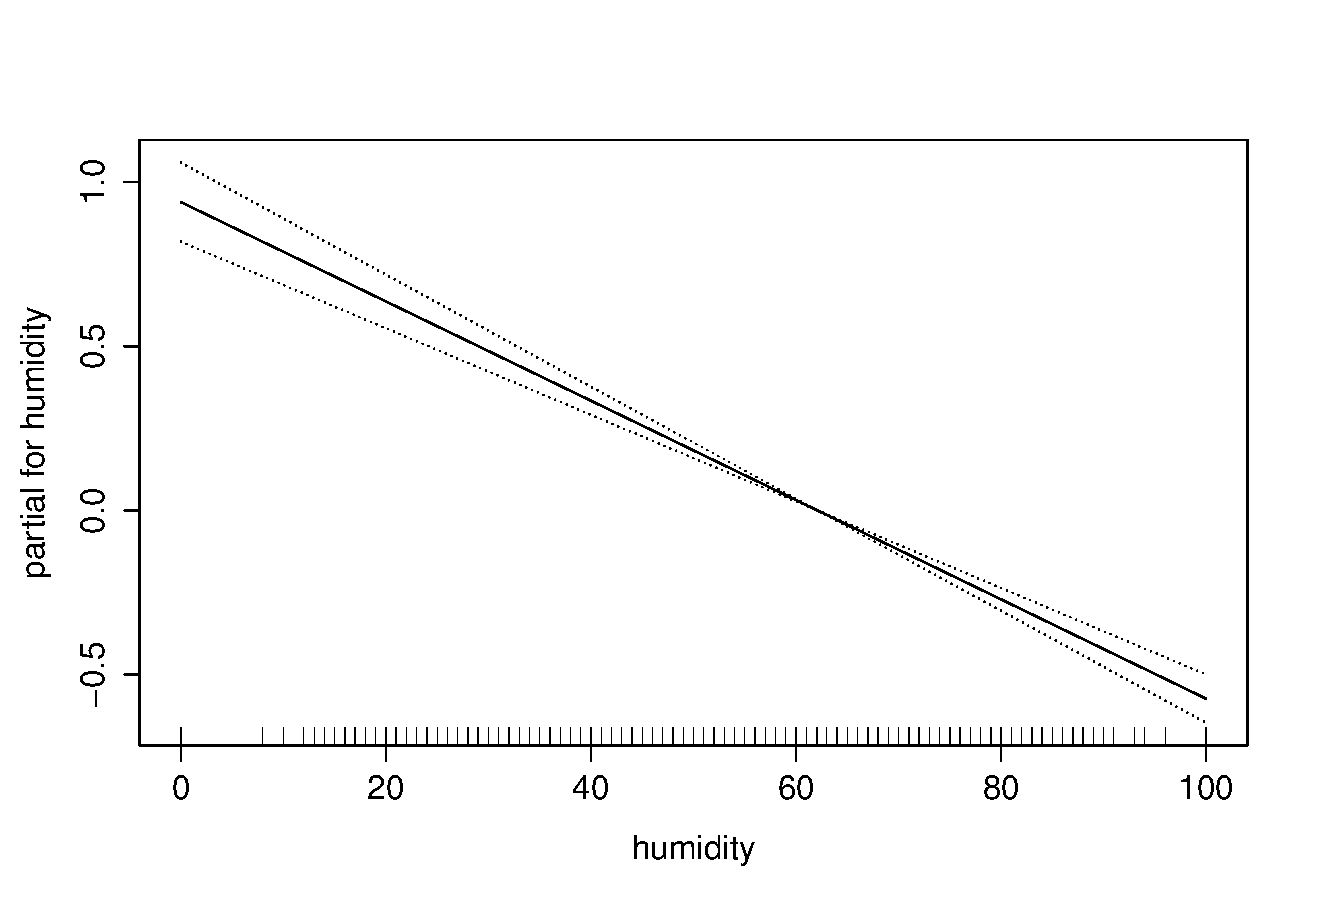
\includegraphics[width=\columnwidth]{images/non-linear/gam/gam-humidity.eps}
        \end{subfigure}

        \medskip
        \begin{subfigure}{0.4\textwidth}
          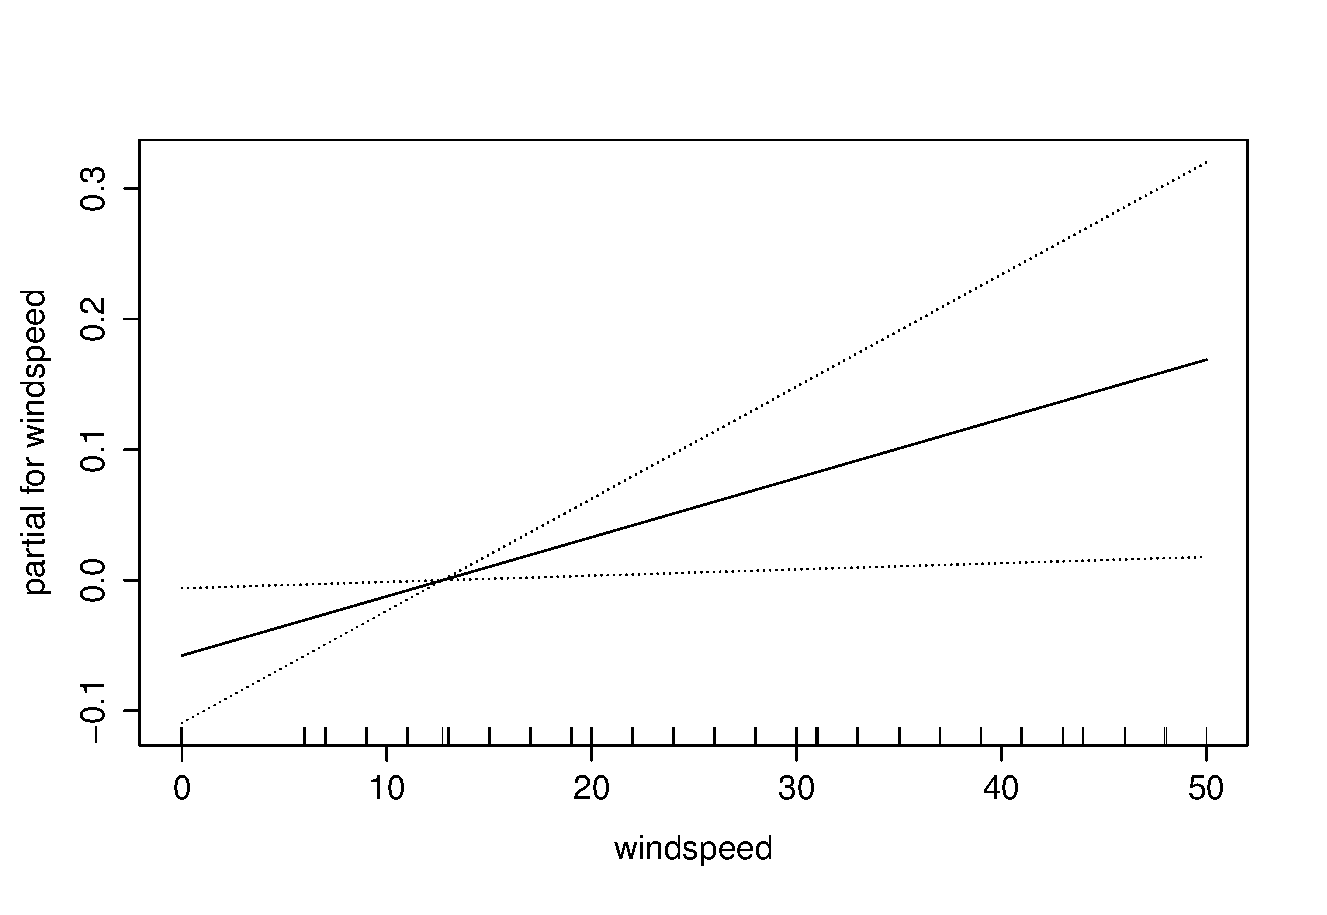
\includegraphics[width=\columnwidth]{images/non-linear/gam/gam-windspeed.eps}
        \end{subfigure}
        \hspace*{\fill}
        \begin{subfigure}{.4\textwidth}
          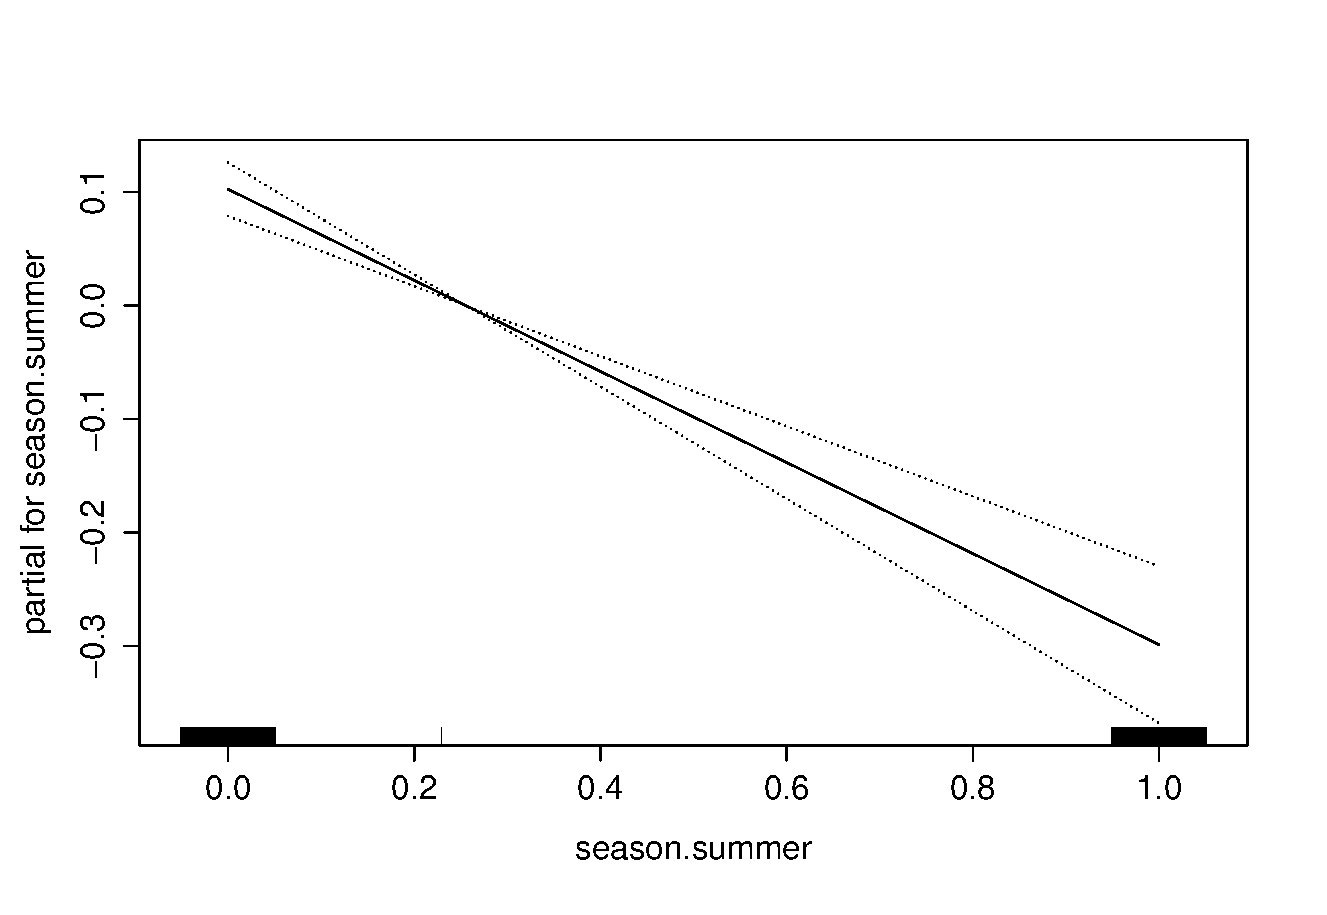
\includegraphics[width=\columnwidth]{images/non-linear/gam/gam-summer.eps}
        \end{subfigure}

        \medskip
        \begin{subfigure}{0.4\textwidth}
          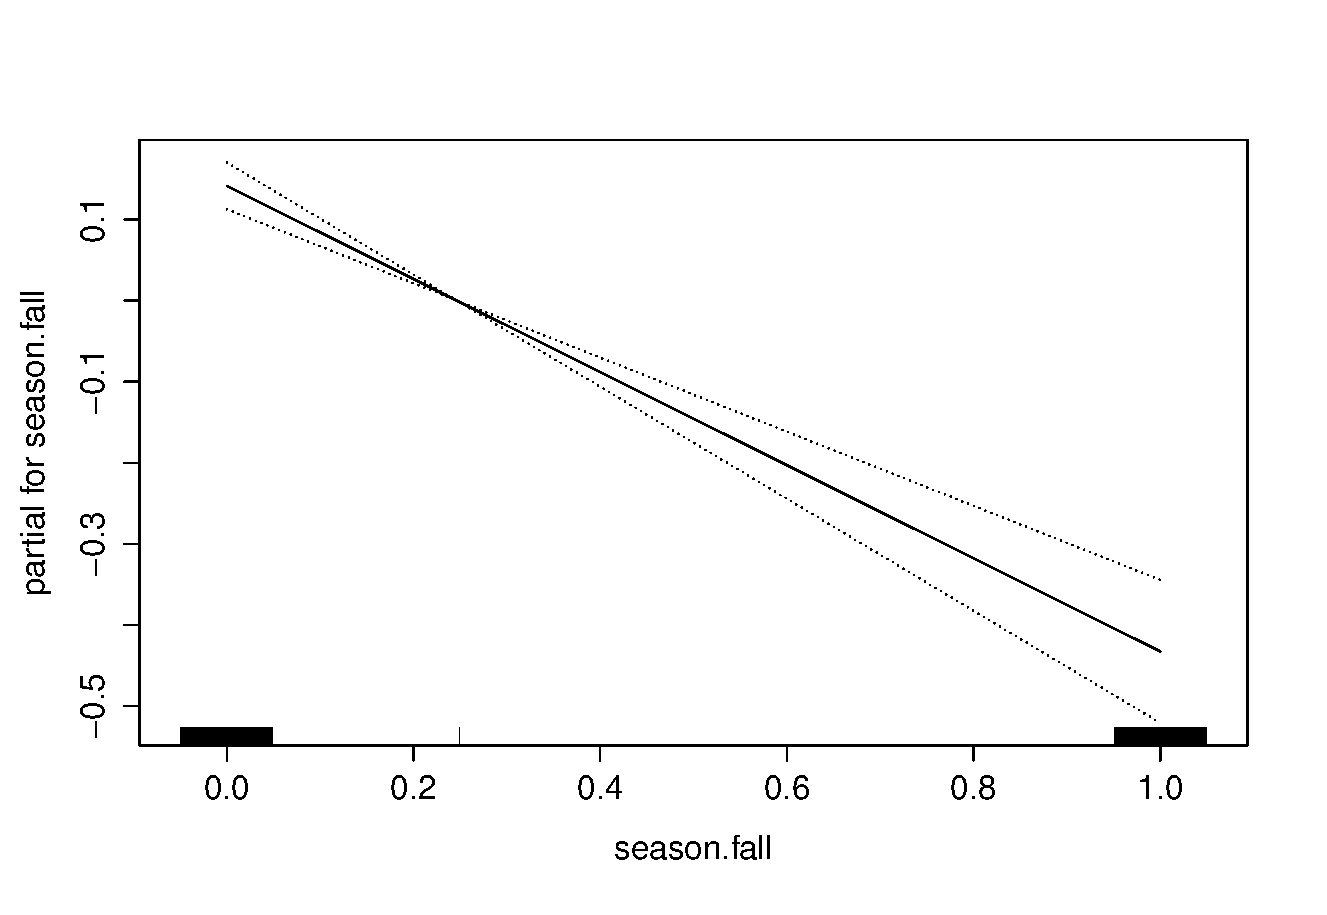
\includegraphics[width=\columnwidth]{images/non-linear/gam/gam-fall.eps}
        \end{subfigure}
        \hspace*{\fill}
        \begin{subfigure}{0.4\textwidth}
          
\includegraphics[width=\columnwidth]{images/blank.eps}
        \end{subfigure}

        \caption{Grafici GAM - 2}\label{fig:gam-1}
\end{figure}

Come è possibile vedere in queste semplici figure, vengono confermati i
risultati visti grazie ai modelli precedenti:

\begin{itemize}
\item \texttt{holiday} era risultata poco significativa nei modelli precedenti
  e nemmeno in questo caso sembra influenzare significativamente la richiesta del servizio;
\item sono stati confermati gli effetti rilevati con i modelli precedenti
  anche per le altre variabili.
\end{itemize}

In questi grafici compare però qualcosa che ci sorprende:

\begin{itemize}
\item Stranamente, al peggiorare del tempo (variabile \texttt{weather}),
  sembra che la richiesta del servizio di \emph{Bike sharing} cresca. \\
  Questa ``anomalia'' potrebbe essere spiegata dal fatto che a Brooklyn al
  peggiorare del tempo le metropolitane diventano più affollate e le strade
  più trafficate, poichè si preferisce utilizzare un mezzo piuttosto che
  andare a piedi. \\
  Sembra quindi che, con condizioni metereologiche accettabili, la gente per
  evitare il traffico o servizi pubblici troppo affollati, preferisca
  ricorrere al servizio di \emph{Bike sharing} piuttosto che camminare per
  qualche isolato.
\item Dalle figure relative alla variabile \texttt{season} pare che il
  servizio di \emph{Bike sharing} venga utilizzato prevalentemente in inverno,
  mentre ci si aspetterebbe che venisse utilizzato maggiormente in estate.
  Tuttavia, facendo qualche ricerca su Internet\footnote{
  https://weatherspark.com/averages/31081/New-York-United-States e altri siti}
  sembra che a Brooklyn in estate il tempo non sia particolarmente gradevole:
  molti lo descrivono come afoso ed è stata trovata una notizia di un ciclista
  di un TG locale in cui egli denuncia che in estate non si riesce più ad
  andare in bici poichè le ruote diventano troppo \emph{slippery}, ovvero
  sdrucciolevoli. \\
  Questa notizia può sembrare realistica poichè guardando la mappa delle piste
  ciclabili\footnote{http://www.nycbikemaps.com/maps/brooklyn-bike-map/} molte
  di queste sono in mezzo a grattacieli ed edifici e solo una piccola parte di
  questi è adiacente al Brooklyn Botanic Garden.
\end{itemize}

Per quanto riguarda gli altri risultati ottenuti, sembrano tutti rispecchiare
alcune previsioni che potrebbero essere ritenute ``comuni'':

\begin{itemize}
\item Al crescere della temperatura, il servizio viene utilizzato di più (per
  rinfrescarsi);
\item Al crescere della velocità del vento, il servizio viene utilizzato di
  più (ci si rinfresca di più se c'è più vento);
\item Al crescere dell'umidità, il servizio viene richiesto di meno (è più
  fastidioso andare in bici con maggiore afosità);
\item Se è un giorno lavorativo, il servizio viene utilizzato di meno poichè
  c'è meno gente che fa un giro in bici;
\item Di notte ci si aspetta che il servizio non venga utilizzato molto, per
  cui il risultato relativo alle ore rispecchia questa previsione.
\end{itemize}

%%%%%%%%%%%%%%%%%%%%%%%%%%%%%%%%%%%%%%%%%%%%%%%%%%%%%%%%%%%%%%%%%%%%%%%%%%%%%%%

\subsection{Projection Pursuit Regression}\label{sec:ppr}
Un altro possibile modello è la \emph{Projection Pursuit Regression}, in cui i
parametri da determinare sono i vettori di proiezione.

In questo modello bisogna ricercare il numero migliore di proiezioni da
utilizzare. Fortunatamente, questo è abbastanza semplice da trovare tramite
iterazioni assegnando a questo numero valori da 1 a un limite superiore
finchè, calcolando lo squarto quadratico, non si trova un minimo: l'andamento
dell'errore infatti è assimilabile ad una funzione che decresce, toccando un
minimo, per poi crescere nuovamente e stabilizzarsi asintoticamente.

Con lo script \texttt{ppr.R} (sez. \ref{sec:ppr-script}) si è notato che basta
iterare al massimo venti volte per arrivare a convergenza con il nostro
dataset.

\begin{figure}[H]
        \begin{subfigure}{0.4\textwidth}
          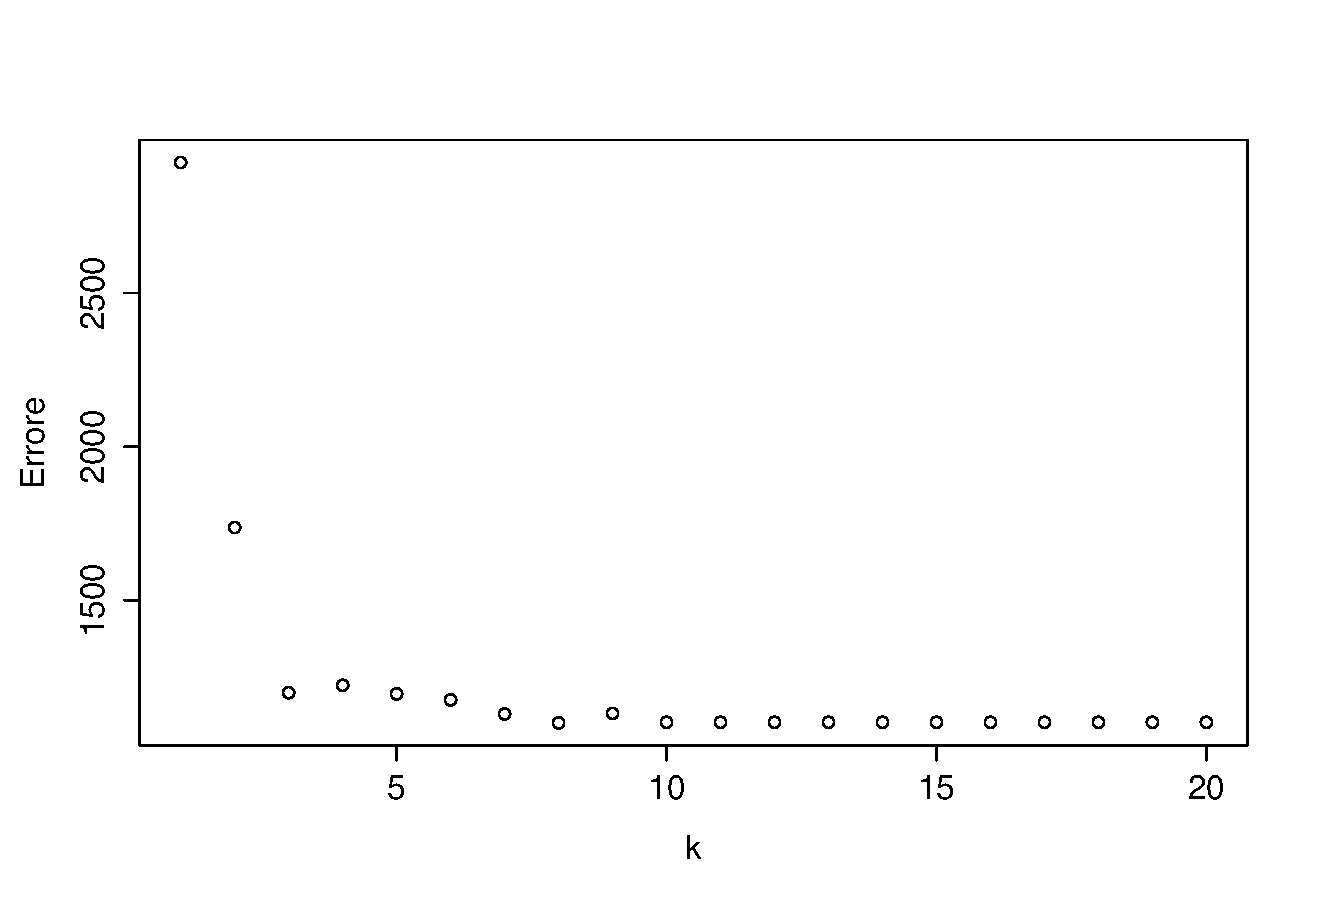
\includegraphics[width=\columnwidth]{images/non-linear/ppr-error-plot.eps}
        \end{subfigure}
        \hspace*{\fill}
        \begin{subfigure}{0.4\textwidth}
          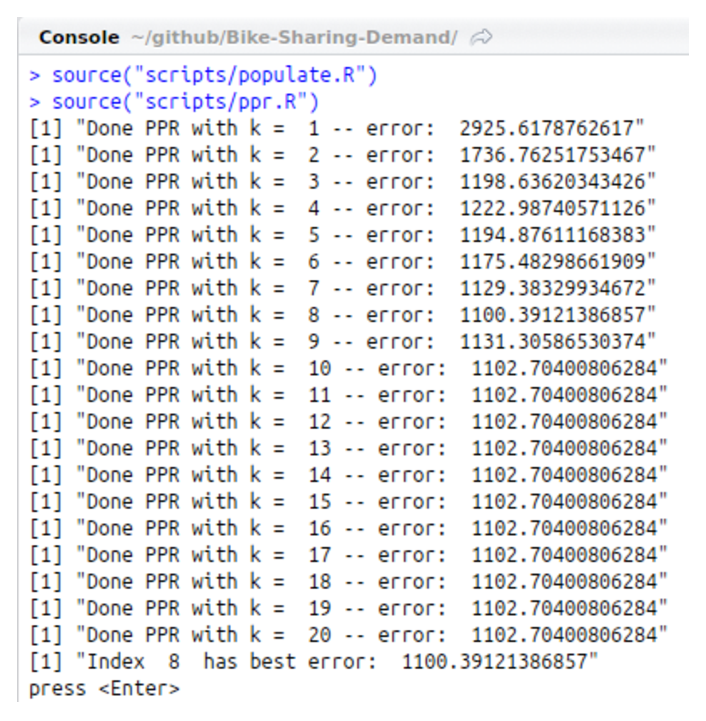
\includegraphics[width=\columnwidth]{images/non-linear/ppr-error-data.eps}
        \end{subfigure}

        \caption{Errore con PPR}\label{fig:ppr-error}
\end{figure}

\begin{figure}[H]
  \centering
  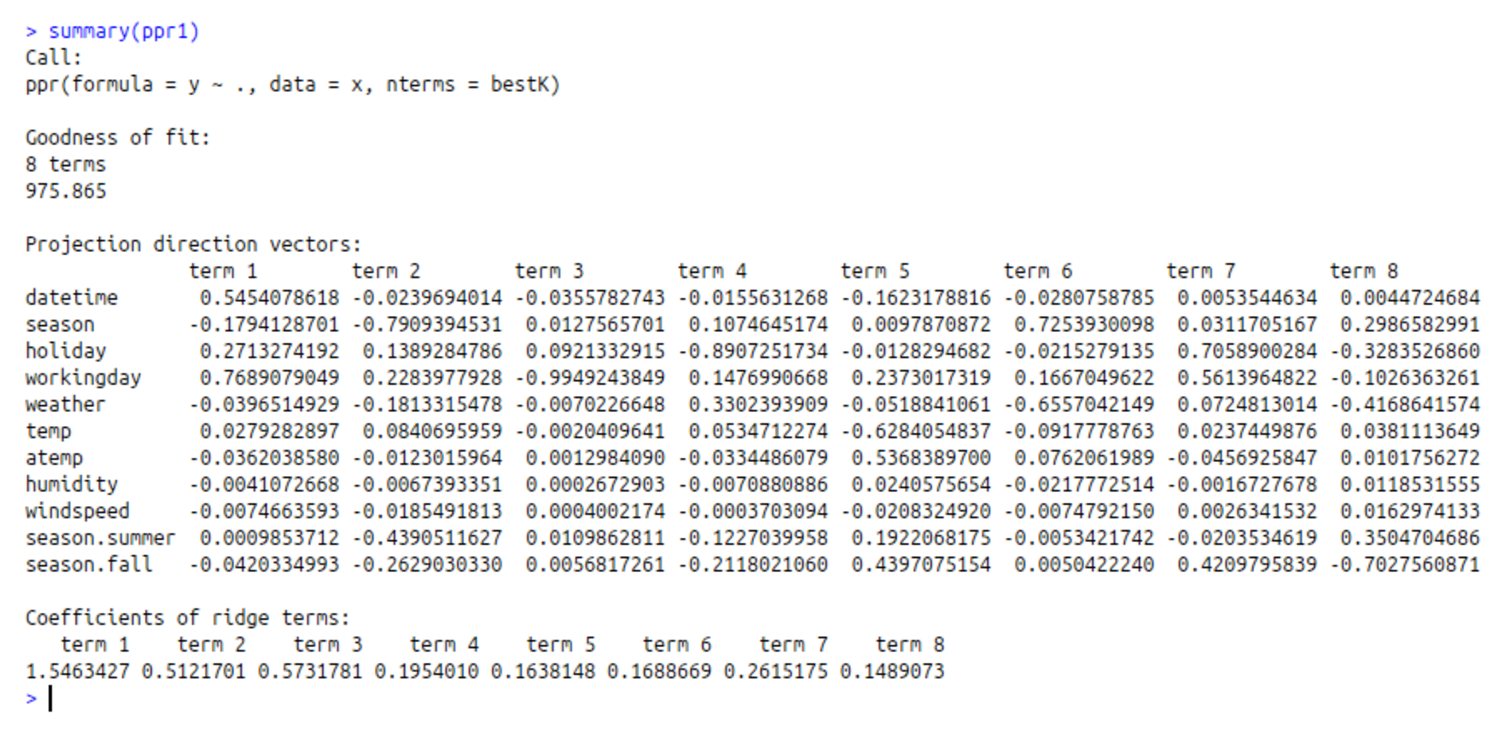
\includegraphics[width=.7\columnwidth]{images/non-linear/ppr-result.eps}
  \caption{Project Pursuit Regression con il miglior numero di proiezioni}
  \label{fig:ppr-result}
\end{figure}

%%%%%%%%%%%%%%%%%%%%%%%%%%%%%%%%%%%%%%%%%%%%%%%%%%%%%%%%%%%%%%%%%%%%%%%%%%%%%%%

\subsection{Reti neurali}\label{sec:neural-nets}
Un altro modello provato per spiegare i nostri dati sono le reti neurali, le
quali hanno l'interessante caratteristica di poter approssimare bene qualsiasi
funzione continua semplicemente aumentando il numero di nodi nello strato
latente.

Naturalmente per utilizzare le reti neurali le funzioni di attivazione non sono
entrambi lineari, altrimenti il tutto si sarebbe ridotto a quanto già visto
nella sezione \ref{sec:linear-model} e nelle relative sottosezioni.

Lo script che si occupa di individuare una rete neurale adatta al nostro
dataset è \texttt{neural-network.R} (sez. \ref{sec:nnet-script}), il quale
fa iterare 100 volte (facendo girare lo script, è stato notato che è un numero
sufficiente grande) per arrivare a convergenza. Per il parametro \emph{decay}
è stato utilizzato 0.0016.

\begin{figure}[H]
  \centering
  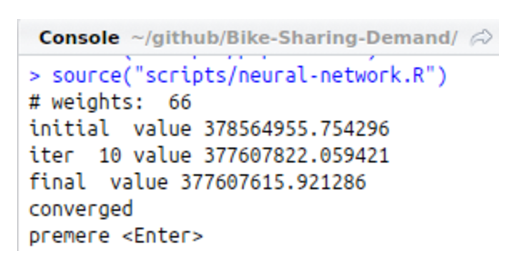
\includegraphics[width=.7\columnwidth]{images/non-linear/nnet-progress.eps}
  \caption{Convergenza durante il calcolo della rete neurale}
  \label{fig:nnet-progress}
\end{figure}

\begin{figure}[H]
  \centering
  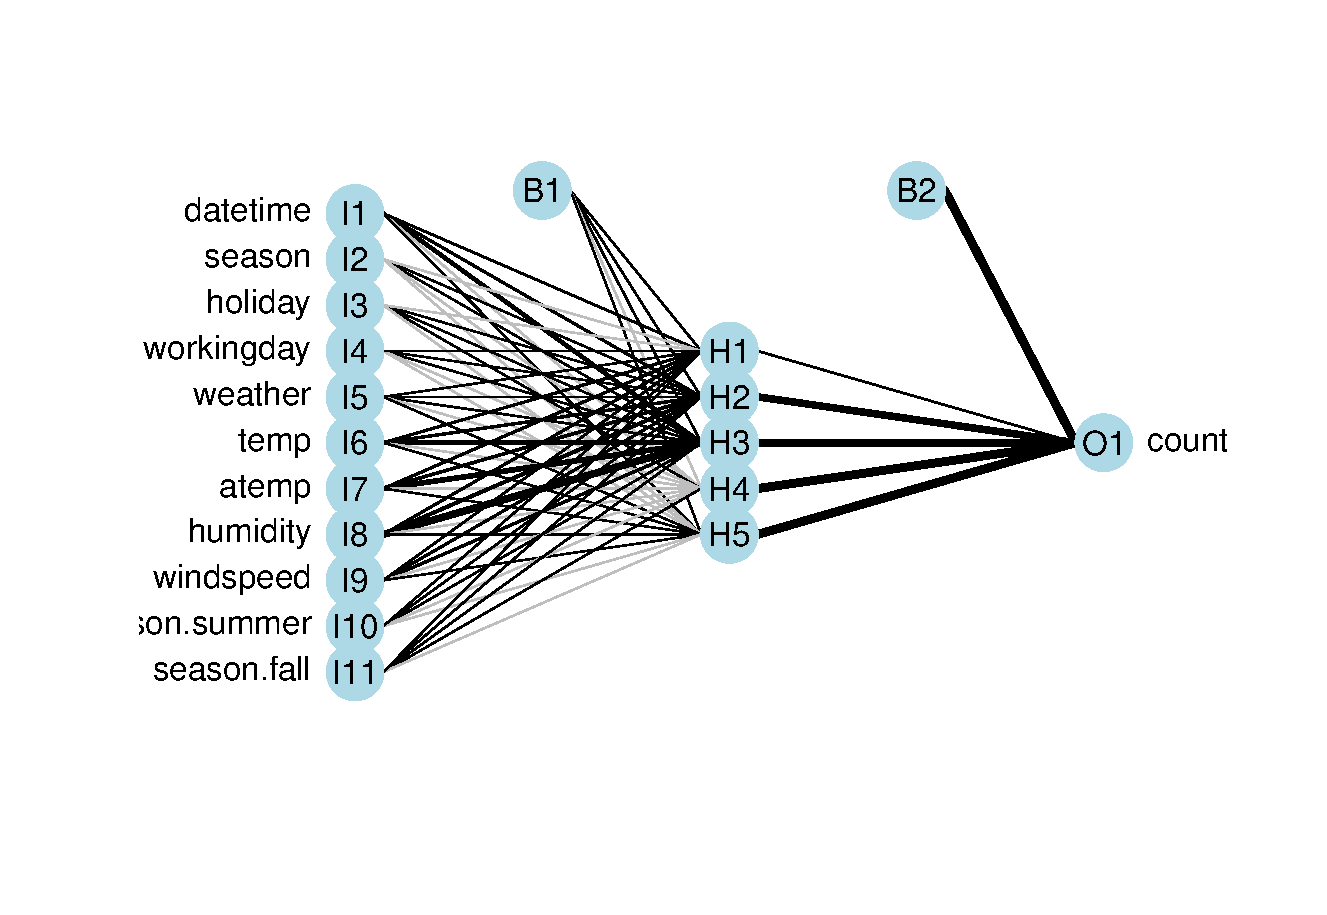
\includegraphics[width=.7\columnwidth]{images/non-linear/neural-network.eps}
  \caption{Rete neurale finale}
  \label{fig:nnet}
\end{figure}
